\documentclass{article}
\usepackage[usenames,dvipsnames]{xcolor}
\usepackage{tcolorbox}
\usepackage{tabularx}
\usepackage{array}
\usepackage{colortbl}
\tcbuselibrary{skins}
\usepackage{graphicx}


\newcolumntype{Y}{>{\raggedleft\arraybackslash}X}

\tcbset{tab1/.style={fonttitle=\bfseries\large,fontupper=\normalsize\sffamily,
colback=yellow!10!white,colframe=red!75!black,colbacktitle=Salmon!40!white,
coltitle=black,center title,freelance,frame code={
\foreach \n in {north east,north west,south east,south west}
{\path [fill=red!75!black] (interior.\n) circle (3mm); };},}}

\tcbset{tab2/.style={enhanced,fonttitle=\bfseries,fontupper=\normalsize\sffamily,
colback=yellow!10!white,colframe=red!50!black,colbacktitle=Salmon!40!white,
coltitle=black,center title}}

% if you need to pass options to natbib, use, e.g.:
%     \PassOptionsToPackage{numbers, compress}{natbib}
% before loading neurips_2021

% ready for submission
\usepackage{neurips_2021}

% to compile a preprint version, e.g., for submission to arXiv, add add the
% [preprint] option:
%     \usepackage[preprint]{neurips_2021}

% to compile a camera-ready version, add the [final] option, e.g.:
%     \usepackage[final]{neurips_2021}

% to avoid loading the natbib package, add option nonatbib:
%    \usepackage[nonatbib]{neurips_2021}

\usepackage[utf8]{inputenc} % allow utf-8 input
\usepackage[T1]{fontenc}    % use 8-bit T1 fonts
\usepackage{hyperref}       % hyperlinks
\usepackage{url}            % simple URL typesetting
\usepackage{booktabs}       % professional-quality tables
\usepackage{amsfonts}       % blackboard math symbols
\usepackage{nicefrac}       % compact symbols for 1/2, etc.
\usepackage{microtype}      % microtypography
\usepackage{xcolor}         % colors

\title{An Autoencoder Neural Network for Precision Oncology and Cancer Data Integration}

% The \author macro works with any number of authors. There are two commands
% used to separate the names and addresses of multiple authors: \And and \AND.
%
% Using \And between authors leaves it to LaTeX to determine where to break the
% lines. Using \AND forces a line break at that point. So, if LaTeX puts 3 of 4
% authors names on the first line, and the last on the second line, try using
% \AND instead of \And before the third author name.



\begin{document}
\maketitle


\begin{abstract}
  Developments in cancer research have led to massive amounts of complex, heterogeneous data. This data is often of very different scale, ranging from molecular to radiological. While advances in cancer and machine learning have led to improvements in diagnosis and treatment of cancer patients, these methods often are trained to analyze variation in individual data types and fail to exploit the inter-dependencies between different data types. Integrating multiple data types is essential in capturing the synergistic nature of biological processes for more accurate prediction and a better understanding of cancer biology. In this paper we demonstrate how an Autoencoder Neural Network for gene expression data can be designed, built and, in particular, applied to gene expression data from the TCGA Stomach Adenocarcinoma Cancer Project.

\end{abstract}

\newpage
\section{Introduction}

Cancer endures as an important threat to human lives. Late diagnosis of cancer contributes largely to its high mortality rate. For example, when stage one breast cancer has a survival rate of 95\%, but this falls to 20\% in stage four (Young et al., 2020). Hence, improving early detection processes is imperative to reducing mortality.

Machine learning methods have shown great potential in improving the diagnostic process. These techniques can uncover underlying patterns in complex data and use them to predict how fast a cancer may progress, or individual patient survival (Korou et al., 2014). For instance, Ayer et al. (2010) found that Artificial Neural Networks could be used to predict malignant breast lesions using mammographic and demographic data from patients. This classification method proved to be superior than those done by radiologists (Ayer et al., 2010). Furthermore, Capper et al. (2018) found that cancer methylome data could be used to build a random forest algorithm that effectively predicted the presence of a wide variety of malignant brain tumors.

Typically, machine learning models for cancer prediction have been developed to address particular complexities inherent in individual data types. While relevant, this approach is sub-optimal because it fails to exploit the inter-dependencies between the different data silos, and is thus often not extendable to analyzing and modeling more complex biological phenomena (Nikola et al., 2019). To design a state of the art machine learning model for precision oncology it is clear that inputs should include data of multiple types, ranging from  molecular to clinical and radiological data, to capture the biological synergies that would be missed by using only one data type. 

One such technique that has shown promise to bring all of these data types together are autoencoders. An autoencoder is an unsupervised machine learning technique that first compresses and then decompresses input data. Specifically, it transforms the input data into a lower-dimensional space and then learns to reconstruct it so that the output is as close to the input as possible. One of the primary objectives of autoencoding is to generate a version of the input data that focuses on the most important features of it, removing inherent noise and lowering the latent dimensionality of the data.

In this paper, we demonstrate how these autoencoder neural  networks can be designed, built, and, in particular, applied to gene expression data for integrative analyses of heterogeneous cancer data. 

\section{Methodology}

\subsection{Data}
Our data comes from the NCI Genomic Data Commons at the University of Chicago (Grossman et al., 2016). The NCI's Genomic Data Commons provides the cancer research community with a unified repository and cancer knowledge base that enables data sharing across cancer genomic studies in support of precision medicine. More specifically, we use RNA-seq data from the TCGA stomach adenocarcinoma cancer project for 137 female patients.


\subsection{Data Pre-Processing}

We begin by linking all 137 female RNA-seq counts to create a single data frame where each row is a patient sample and the columns represent the counts of expressed genes. Since the vast majority of the biology of a genome is initially inferred from the set of proteins that genome is predicted to encode, we further limit our sample to only genes that are protein coding genes. Given our small number of samples of stomach adenocarcinoma cancer, using only protein coding genes allows us to limit our feature space from 60,483 genes to 19,561 genes. 

The nominal counts of each gene expression may not be as important as is the distribution of genes from a given cancer sample. Thus, we normalize each row of our data such that each value is the proportion of that gene expression as compared to the sum of all genes expressed. Therefore, the range of all of our features falls between 0 and 1. Finally, our data was randomly divided in two groups: training set (70\%) and test set (30\%). The training set is used to design our encoding and decoding function, and the test set is used to validate our model and compute our model's losses/error.   


\subsection{Autoencoders}

In nearly all contexts where the term "autoencoder" is used, the compression and decompression functions are implemented through Artificial Neural Networks (ANN). An ANN refers to a set layers of interconnected nodes. Figure 1 shows an illustration. For this example, each node is represented by a circle and each layer is represented by a column of circles. The first layer to the left represents the input of the encoder, the middle layer is called the 'bottleneck', and the last layer to the right represents the output of the ANN. 

Figure 1 depicts a network with five layers, four input features (\begin{math}X_1, X_2, X_3, X_4\end{math}), and two nodes in the bottleneck layer. It can be seen how the inputs are transformed into layers of lower dimensions/nodes (encoded) until they reach the bottleneck. The nodes in the bottleneck are then decoded into higher dimensions until they reach the original dimension of the input. 

\begin{figure}[h]
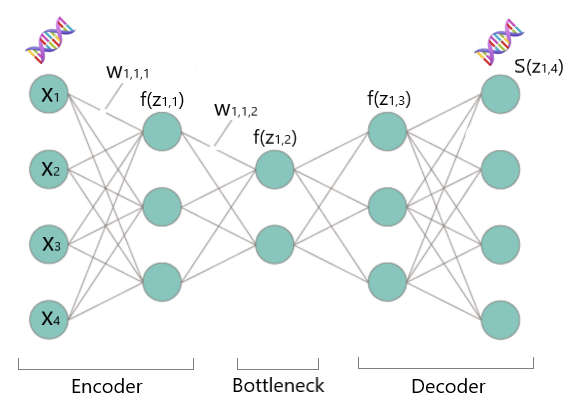
\includegraphics[width=10cm]{NN_decoder.png}
\centering
\caption{Autoencoder Neural Network Architecture}
\end{figure}

The edges that connect nodes between layers represent a weight (\begin{math}W_{i,j,k}\end{math}), where $i$ refers to the within-layer number of the origin, $j$ refers to the within-layer number of the destiny, and $k$ represents the layer of the origin. Under this notation, (\begin{math}W_{2,3,1}\end{math}) would refer to the weight that starts from the first layer $(k = 1)$, specifically from \begin{math}X_2\end{math} $(i = 2)$, and ends in the third node $(j = 3)$ of the second layer. As it can be seen, every node is connected to every other node in the layers that are contiguous to each other. This means that every node in layer $k$ will be used to compute every node in layer $k+1$. The way previous nodes are used to create these new nodes is through the activation function  \begin{math}f()\end{math}. For example, the nodes from the second layer would adhere to the following equation: 

\begin{equation}
    f(Z_{j,1}) = f(\ W_0 + X_1W_{1,j,1} + X_2W_{2,j,1} + X_3W_{3,j,1} + X_4W_{4,j,1})
\end{equation}


where \begin{math}Z_{j,1}\end{math} is the linear combination of all of the nodes in the previous layer (\begin{math}X_1, X_2, X_3, X_4\end{math}) weighted by \begin{math}W_{1,j,1}, W_{2,j,1}, W_{3,j,1}, W_{4,j,1}\end{math} plus a constant \begin{math}W_0\end{math}. This suggests that, to compute each node of the second layer, we need to estimate 5 parameters (4 previous nodes plus a constant). It is easy to see that the number of parameters that need to be estimated for a network increases rapidly with the number of nodes and layers.  

An ANN needs a loss function to estimate its parameters. In the case of an autoencoder, this loss function will compare the output of the network with its input and calculate how different they are from one another. The choice of a loss function, as well as the activation function, should be done according to the type of data being used and the purpose of the project. 

The estimation process of an ANN is usually implemented through two algorithms: Stochastic Gradient Descent (SDG) and Backpropagation. In short, SDG is implemented by following these steps:

\begin{enumerate}
   \item Each weight \begin{math}W_{i,j,k}\end{math} is assigned an initial arbitrary (commonly random) value. 
   \item Based on these weights, the output and the loss of the output are computed.
   \item Using a subset of the all of the samples (i.e. a batch), we estimate the gradients of the loss function. This would result in one gradient for each parameter that requires estimation. 
   \item Based on all of these gradients, we adjust the value of our parameters so that they fall closer to the minimum loss.
   \item We repeat steps 2 through 4 and stop only when the gradients are small enough. 
 \end{enumerate}

Backpropagation is particularly useful to an ANN and it happens in step 4 when we calculate the gradients of the weights closer to the output first and those closer input last. The process of updating the set of weights in an ANN (e.g. steps 2-4) is called an epoch. 
 
\section{Estimation}

In practice, it is hard to know ex ante which number of layers, bottleneck size, or activation function will be optimal for an  ANN. Therefore, it is necessary to experiment with these parameters and choose those that achieve the goals of your application. For our data, we varied these parameters and compared the performance of several autoencoder models. More specifically, we varied the following parameters:

\begin{itemize}
  \item Bottleneck size: we varied the number of nodes in our middle layers from a minimum of 10 to a maximum of 100.
  \item Number of layers: 5, 7 and 9 layers. 
  \item Activation function: we tested three different activation functions for most of our nodes: Linear, Rectified Linear Unit (ReLU) and Sigmoid. The formal definitions for each of these functions are made explicit below:  
\end{itemize}

\begin{equation}
    Linear = L(x) =  x
\end{equation}
\\
\begin{equation}
    ReLU = R(x) =  max(0, x)
\end{equation}
\\
\begin{equation}
    Sigmoid = S(x) =  \frac{\mathrm{1} }{\mathrm{1} + e^{-x} } 
\end{equation}

As it can be seen, the linear function would leave our nodes as a weighted combination of our weights and the previous nodes plus the constant. ReLU, on the other hand, would do the same thing, unless $x$ was less than zero. If that was the case then it would return $0$. Finally, Sigmoid is a function that guarantees that its output will be between 0 and 1. Given this useful property and the fact that our input is also always between this range, we have set the activation functions of our last layer to be Sigmoid. So even when tuning our activation functions, the last layer's Sigmoid will stay constant. 

For our loss function, we have chosen to use a Binary Cross-Entropy loss:

\begin{equation}
    - (y* log(p)+(1-y)*log(1-p))
\end{equation}

where \begin{math}y\end{math} is the original input and $p$ is the output of the autoencoder. Although this function was made for binary classification tasks, it can also be leveraged for our purposes and provide us with a useful measure of similarity between inputs and outputs. This is largely due to the range of our inputs/outputs which go from $0$ to $1$.  

Finally, since the number of samples in our dataset is $137$, we set our batches to $10$ and the number of epochs to $40$. We found that increasing the number of epochs further did not change our results significantly. 

\section{Results and Discussion}

The results of these estimations are summarized in Figure 2 in the Appendix. In this graphic, the vertical axis represents the loss value of each auto-encoder on the test set. Since the objective of the ANN is to minimize said function, lower values for this axis are preferred. The horizontal axis represents the number of nodes that were in the middle layer of the autoencoder. The colors of each line refer to the activation function that was used, while the pattern of the line refers to number of layers incorporated. 


As shown, the autoencoders with only $5$ layers (solid pattern) performed the worst and resulted in the highest loss. Additionally, the autoencoders with $9$ layers yield the minimum loss possible, performing slightly better than those with 7 layers. This finding is reasonable: more layers imply that the model has to estimate more parameters and that the complexities of the data could be better explained. Hence, there is an inverse relationship between the number of layers and the loss. Although this argument would also apply to the size of the bottleneck, we did not find a significant decrease in the loss values as bottleneck size increased, which is puzzling. 

For our activation function, it seems like our three variants performed very similarly when trained in a 7 to 9 layer network. However, the activation function that yielded the minimum loss value was Sigmoid when coupled with 9 layers.

Finally, Figure 3 provides an overall picture of the differences between the input and output of the best-performing auto-encoder. To create this, we estimated the first and second principal components of both our raw input and auto-encoded output. Principal components are linear combinations of the original features and the first two correspond to the two directions of greatest variance within our data. Therefore, the first two components will not display all of the variance inherent in our data, but they will give us a glimpse into the nature of each set and will allow a very basic visual comparison.


As the figure suggests, the first two principal components of our output seem to behave very different than those of our input data. So although our ANN was trained to minimize the difference between both of them, the two directions of greatest variance of both differ dramatically. This is not enough to suggest anything regarding the usefulness of autoencoders for precision oncology. For this, we would need to test which dataset (the raw input or the encoded one) is better at predicting cancer patients. Nevertheless, it provides a simple visual inspection technique that could help us understand the differences between our input and output.

\newpage 

\section*{References}

{
\small

[1] Alexander, J.A.\ \& Mozer, M.C.\ (1995) Template-based algorithms for
connectionist rule extraction. In G.\ Tesauro, D.S.\ Touretzky and T.K.\ Leen
(eds.), {\it Advances in Neural Information Processing Systems 7},
pp.\ 609--616. Cambridge, MA: MIT Press.

[2] Bower, J.M.\ \& Beeman, D.\ (1995) {\it The Book of GENESIS: Exploring
  Realistic Neural Models with the GEneral NEural SImulation System.}  New York:
TELOS/Springer--Verlag.

[3] Simidjievski Nikola, Bodnar Cristian, Tariq Ifrah, Scherer Paul, Andres Terre Helena, Shams Zohreh, Jamnik Mateja \ \& Liò Pietro \ (2019) Variational Autoencoders for Cancer Data Integration: Design Principles and Computational Practice . {\it Frontiers in Genetics} 10.3389/fgene.2019.01205

[4] Konstantina Kourou, Themis P. Exarchos, Konstantinos P. Exarchos, Michalis V. Karamouzis,  \ \& Dimitrios I. Fotiadis \ (2014) Machine learning applications in cancer prognosis and prediction. {\it Computational and Structural Biotechnology Journal} 10.1016/j.csbj.2014.11.005

[5] Q. Zhou, B. Yong, Q. Lv, J. Shen \ \& X. Wang \ (2020) Deep Autoencoder for Msas Spectometry Fearture Learning and Cancer Detection {\it IEEE Access} 10.1109/ACCESS.2020.2977680

[6] Ayer T, Alagoz O, Chhatwal J, Shavlik JW, Kahn CE Jr \ \& Burnside ES. \ (2010) Breast cancer risk estimation with artificial neural networks revisited: discrimination and calibration {\it Cancer} 10.1002/cncr.25081

[7] Capper, D., Jones, D., Sill, M. et al \ (2018) DNA methylation-based classification of central nervous system tumours. {\it Nature} 555, 469–474 10.1038/nature26000

[8] Grossman, Robert L., Heath, Allison P., Ferretti, Vincent, Varmus, Harold E., Lowy, Douglas R., Kibbe, Warren A., Staudt, Louis M. (2016) Toward a Shared Vision for Cancer Genomic Data. \it{New England Journal of Medicine} 375:12, 1109-1112
}





%%%%%%%%%%%%%%%%%%%%%%%%%%%%%%%%%%%%%%%%%%%%%%%%%%%%%%%%%%%%
\newpage 

\appendix

\section{Appendix}

\begin{figure}[h]
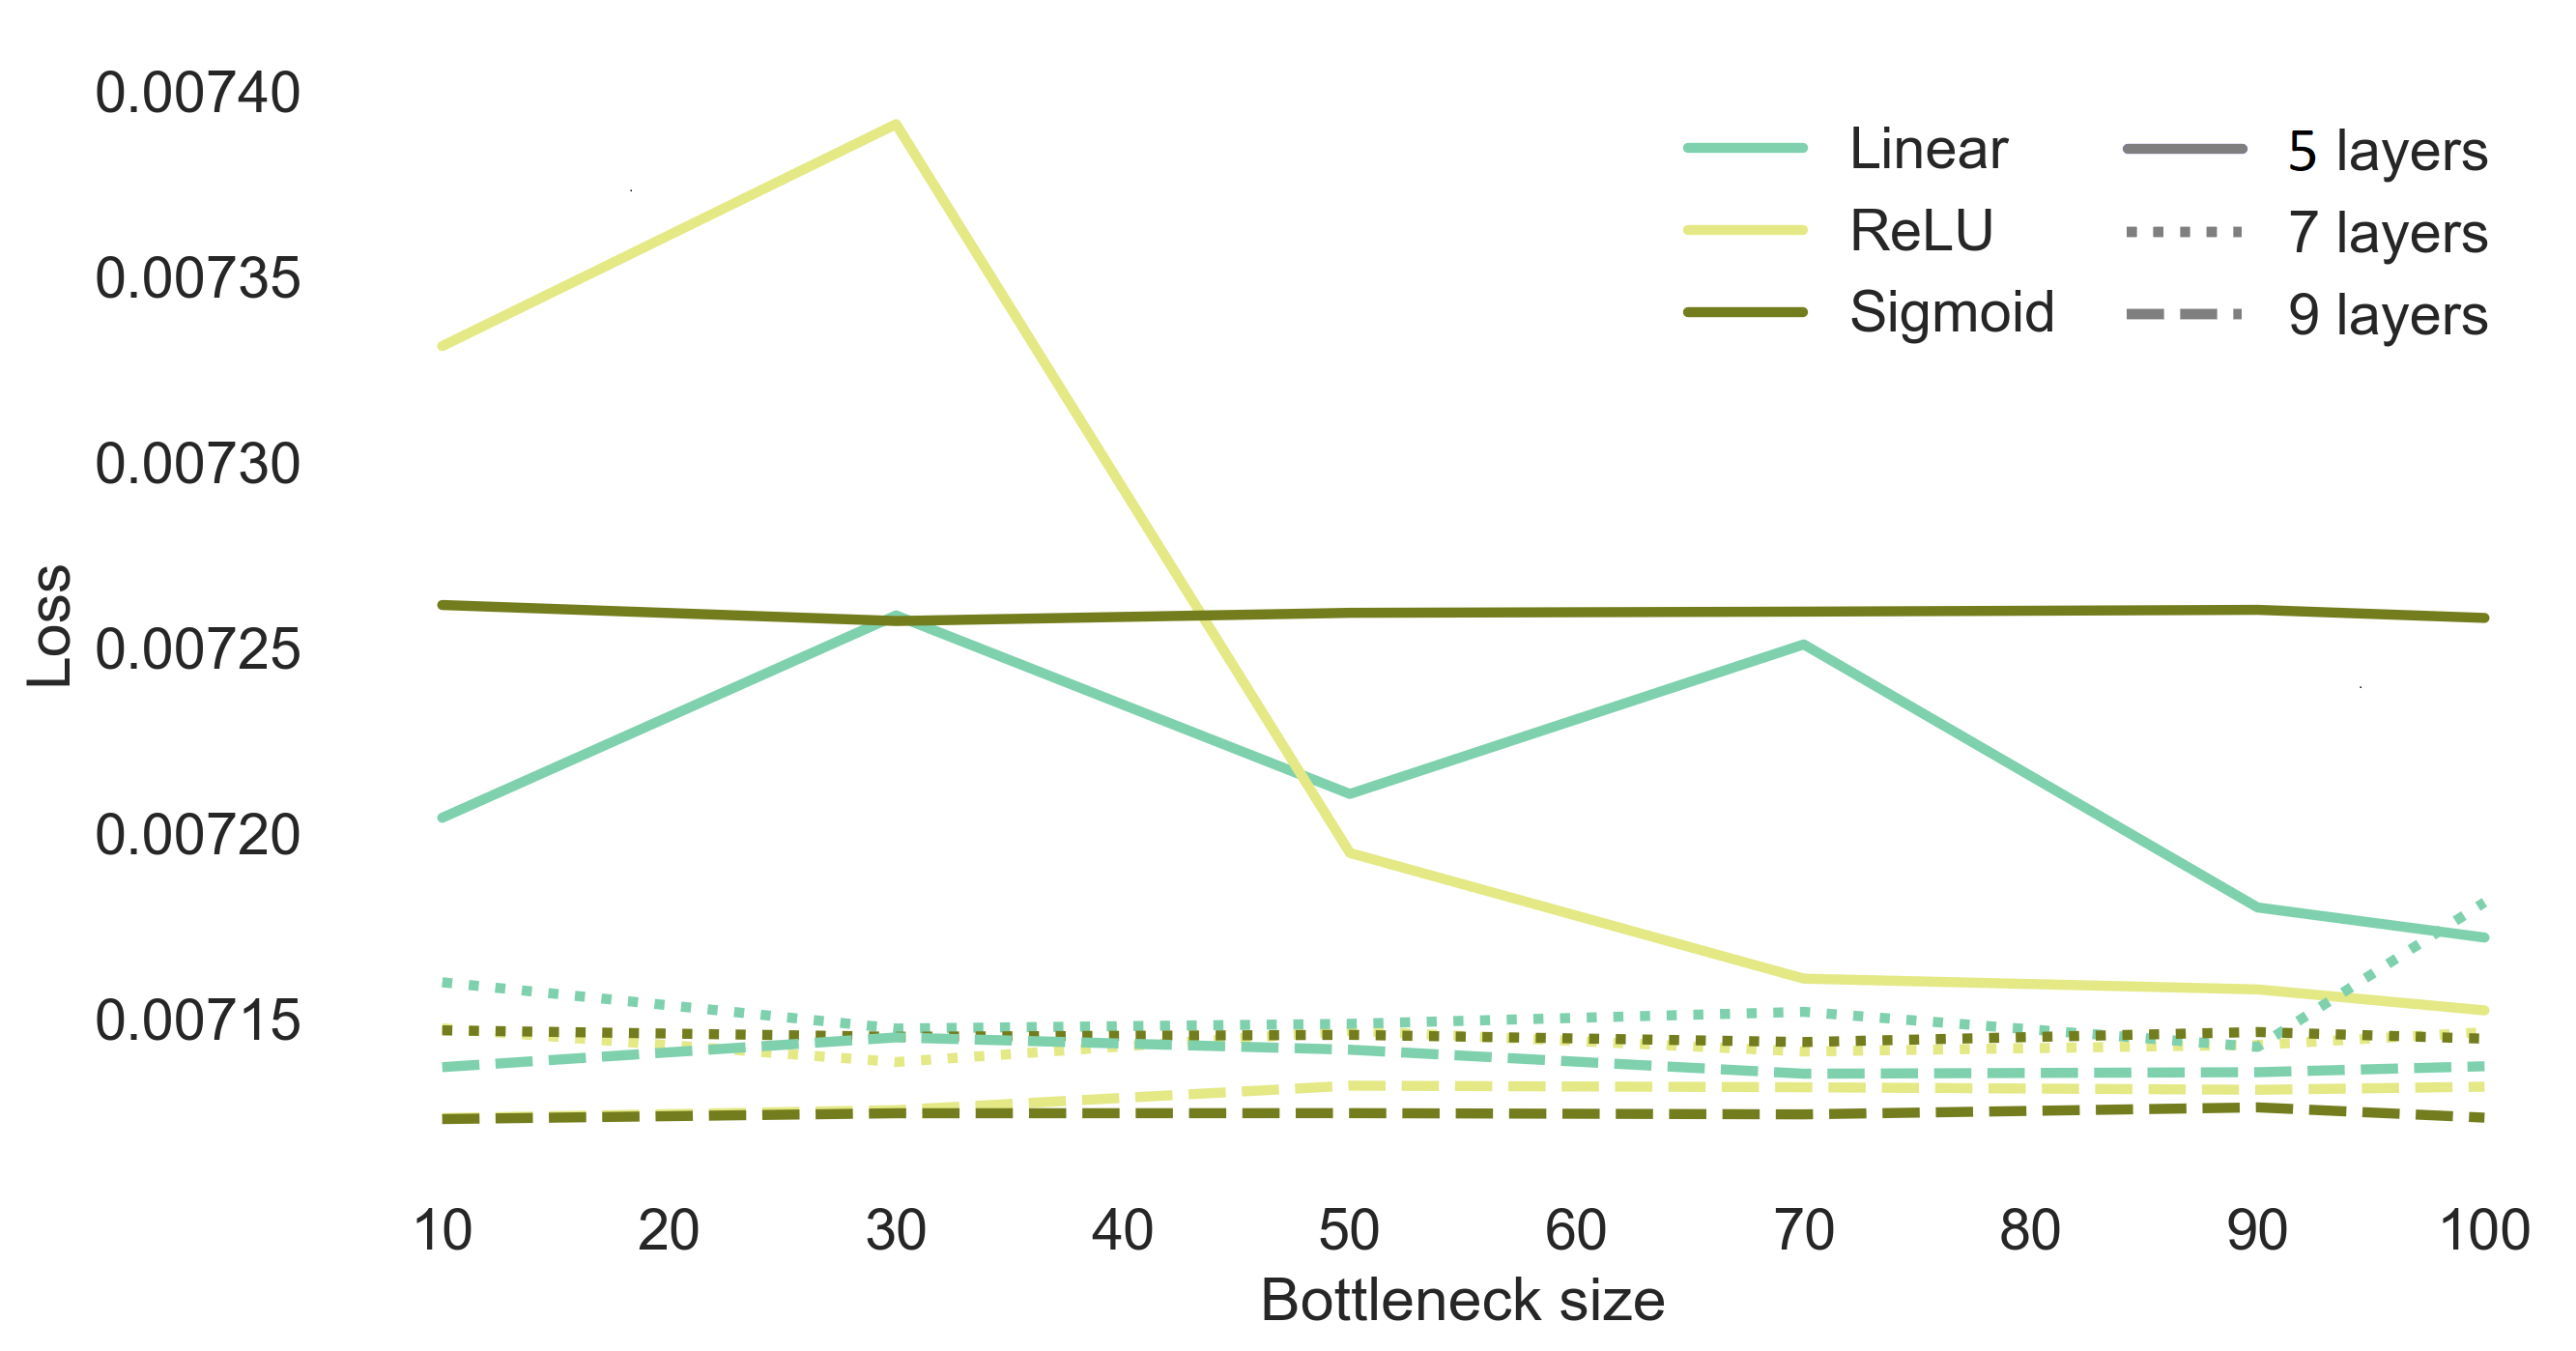
\includegraphics[width=12cm]{NN_lay_act_bsize_loss.png}
\centering
\caption{Encoder Loss by bottleneck size, layers, and activation function}
\end{figure}

\begin{figure}[h]
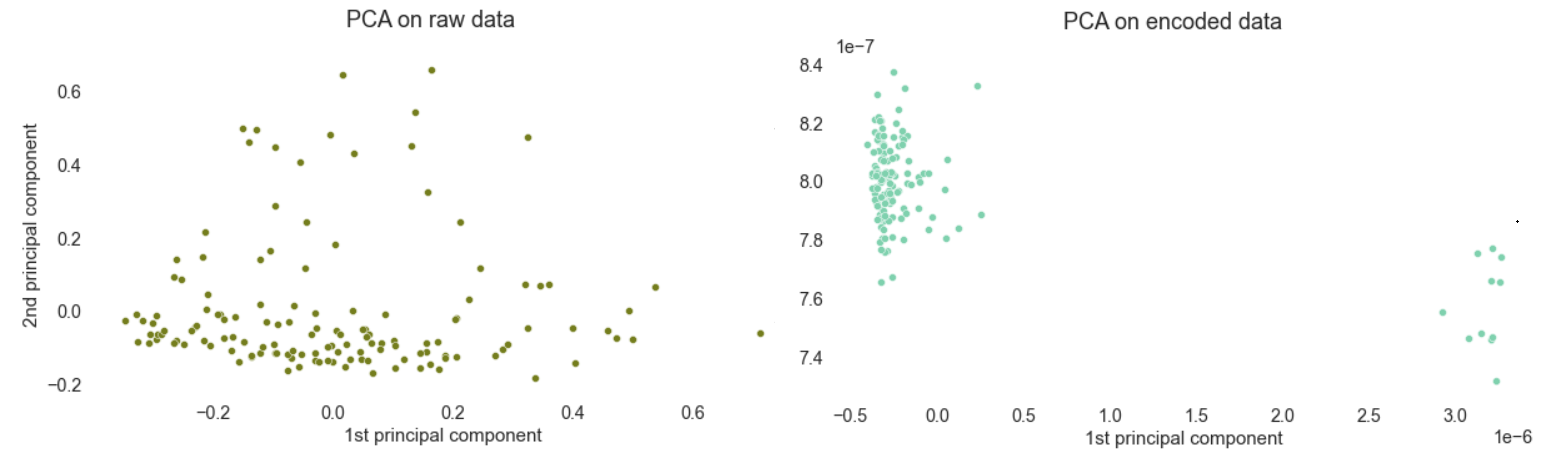
\includegraphics[width=15cm]{PCA_both.png}
\centering
\caption{First two principal components on input and output data}
\end{figure}



\end{document}